\documentclass[
  bibliography=totoc,     % Literatur im Inhaltsverzeichnis
  captions=tableheading,  % Tabellenüberschriften
  titlepage=firstiscover, % Titelseite ist Deckblatt
]{scrartcl}
\usepackage{scrhack}
\usepackage[aux]{rerunfilecheck}
\usepackage{fontspec}
\usepackage[ngerman]{babel}
\usepackage{graphicx}
\usepackage[section, below]{placeins}
\usepackage{caption}
\usepackage{scrlayer-scrpage}
%Mathe Pakete
\usepackage{amsmath}
\usepackage{amssymb}
\usepackage{mathtools}
\usepackage{xfrac}
\usepackage[math-style=ISO,bold-style=ISO,sans-style=italic,nabla=upright,partial=upright]{unicode-math}
\usepackage[
  math-style=ISO,
  bold-style=ISO,
  sans-style=italic,
  nabla=upright,
  partial=upright,
]{unicode-math}
\usepackage[
  locale=DE,
  separate-uncertainty=true,
  per-mode=symbol-or-fraction,
]{siunitx}
\usepackage{subcaption}
\usepackage{graphicx}
\usepackage{booktabs}
\usepackage{microtype}
\usepackage[unicode]{hyperref}
\usepackage{bookmark}
\setmathfont{Latin Modern Math}
\usepackage{csquotes}
\usepackage{wrapfig}
\usepackage[shortcuts]{extdash} % Trennung von Wörtern mit Strichen
\usepackage[backend=biber]{biblatex} %Literaturverzeichnis
\addbibresource{lit.bib}
\usepackage[section]{placeins}%Floats plazieren
\usepackage[version=4, math-greek=default,text-greek=default,]{mhchem} %Chemische Zeichen

\begin{document}
  \setlength{\parindent}{0em} %keine Einrückungen am Zeilenanfang
  \pagestyle{scrheadings}
  \clearpairofpagestyles
  \ofoot{\pagemark}

  \title{V 308 \\Spulen und Magnetfelder}
  \author{Julian Hayduk \and Alex Nuss}
  \date{Durchführung: 22.11.2022, Abgabe: 29.11.2022}
  \subtitle{Versuchsort: TU Dortmund }
  \maketitle

  \thispagestyle{empty}
  \newpage
  
  \tableofcontents


  
  \setcounter{page}{1}
  
  \newpage
  \section{Zielsetzung}
  \label{sec:Zielsetzung}
  
  Ziel des Versuchs ist es die Feldstärken unterschiedlicher Spulen in verschiedenen Anordnungen in
  Abhängigkeit des Ortes zu messen, dazu werden eine lange und kurze Spule, sowie ein Helmholtzspulenpaar verwendet.
  Weiterhin wird mit einer Toroidspule ein Eisenkern magnetisiert und eine
  Hystereskurve dazu graphisch dargestellt.
  
  \section{Theorie}
  \label{sec:Theorie}
  
  Im Allgemeinen erzeugen bewegte Ladungen magnetische Felder. Die magnetische Feldstärke ist eine vektorielle Größe
  und ist durch das Biot-Savart-Gesetz
  
  \begin{equation}
    \label{eqn:magFeldstaerke}
    \vec{H} = \mu_{0}\cdot\mu_{\symup{r}}\cdot \vec{B}
  \end{equation}
  
  beschrieben. Dabei ist $\mu_{0}$ die Vakuumpermeabilität, $\mu_{\symup{r}}$ die materialabhängige relative
  Permeabilität und $\vec{B}$ die magnetische Flussdichte. Die beiden Permeabilitäten lassen sich zu
  $\mu = \mu_0 \cdot \mu_{\symup{r}}$ zusammenfassen. Um die Magnetfeldstärken beliebiger
  Leiterschleifen zu bestimmen, wird das Biot-Savart-Gesetz verwendet, das durch
  
  \begin{equation}
    \label{eqn:biotsavart}
    \vec{B}(r) = \frac{\mu_{0}I}{4\pi} \int_{\Gamma} \frac{\vec{ds}\times \vec{r}}{r^3}
  \end{equation}
  
  gegeben ist. $I$ ist in diesem Fall die Stromstärke und $\Gamma$ der Weg der Schleife. Für eine Spule mit
  $n$ Windungen ergibt sich daraus
  
  \begin{equation}
    \label{eqn:nSpule}
    \vec{B}(x) = \frac{n \mu_0 I}{2} \frac{R^2}{(R^2 + x^2)^{\frac{3}{2}}} \cdot \hat{x}.
  \end{equation}
  $R$ ist dabei der Radius der Spule und $x$ ist der Abstand zum Spulenzentrum. Handelt es sich um eine
  langgestreckte Spule mit Länge $l$, lässt sich die Flussdichte durch
  
  \begin{equation}
    \label{eqn:langeSpule}
    \vec{B}(x) = \mu_{\symup{r}}\mu_0 \frac{n}{l} I
  \end{equation}
  
  beschreiben, da die Feldlinien innerhalb der Spule parallel zur Spulenachse verlaufen.
  (Gleichung 4) gilt nur, wenn die Länge der Spule $l$ viel kleiner als der Durchmesser $d$
  der Spule ist. Wird ein Solenoid nun zu einer Ringspule mit Radius $r_{\symup{T}} << l$ gebogen, fallen die
  Randeffekte weg und die Flussdichte lässt sich nach (Gleichung 4) mit $l = 2\pi r_{\symup{T}}$
 
  \begin{equation}
    \label{eqn:ringspule}
    \vec{B}(r) = \mu_{\symup{r}}\mu_0 \frac{n}{2\pi r_{\symup{T}}} I
  \end{equation}
  
  bestimmen. Damit ein homogenes Magnetfeld erzeugt wird, werden Helmholtz-Spulenpaare verwendet. Dazu werden
  zwei identische Spulen so positioniert, dass ihre Spulenachsen gleich sind und der Abstand der Zentren
  gleich dem Spulenradius $R$ ist. Die schematische Darstellung dafür ist in (Abbildung 1) zu finden.
 
  \begin{figure}
    \centering
    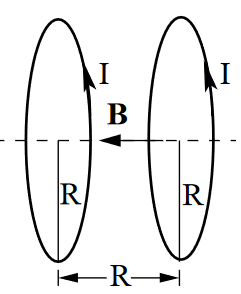
\includegraphics[scale=0.5]{helmholtzspulenpaar.png}
    \caption{Skizze eines Helmholtz-Spulenpaars [1].}
    \label{fig:helmholtz}
  \end{figure}
  
  Die magnetische Flussdichte im Zentrum der Spule lässt sich durch das Biot-Savart-Gesetz bestimmen.
  Die Gleichung für das Helmholtz-Spulenpaar ist dann durch Überlagerung der beiden Felder bestimmt.
  Es ergibt sich
  
  \begin{equation}
    \label{eqn:helmholtz}
    \vec{B}(x) = \frac{n\mu_0 I R^2}{(R^2+x^2)^{\frac{3}{2}}}.
  \end{equation}

  \subsection{Hysteresekurve}
  \label{sec:hysterese}
  
  Befindet sich zusätzlich noch ein ferromagnetischer Stoff in der Spule muss, dessen Magnetisierung $\vec{M}$
  noch bedacht werden. Dieser Umstand lässt sich durch
  
  \begin{equation}
    \vec{B} = \mu_0 (\vec{H} + \vec{M})
  \end{equation}
  
  ausdrücken. Ferromagnetische Stoffe haben sogenannte Weiß'sche Bezirke, in denen die magnetischen
  Momente parallel zueinander ausgerichtet sind. In unmagnetisierten Materialien sind diese statistisch verteilt,
  sodass ferromagnetische Stoffe ein permanentes magnetisches Moment besitzen.\\
  Wird nun ein externes Magnetfeld angelegt, richten sich die magnetischen Momente der Weiß'schen Bezirke
  nach der Richtung des Magnetfelds aus, bis das Gesamtfeld einen Sättigungswert 
  $B_{\symup{S}}$ erreicht. Wird das Magnetfeld nun abgeschaltet, bleibt eine Restmagnetisierung
  über, die Remanenz genannt wird. Um diese auszugleichen, kann ein magnetisches Feld, das
  auch Koerzitivkraft $H_{\symup{C}}$ genannt wird, aufgewandt werden. Nach weiterem Erhöhen des Gegenfelds
  erreicht die Kurve den Sättigungswert $-B_{\symup{s}}$. Wird nun das Feld umgekehrt und erhöht, ergibt sich eine
  symmetrische Kurve zum Ursprung, die schematisch in (Abbildung 2) dargestellt ist.
  
  \begin{figure}
    \centering
    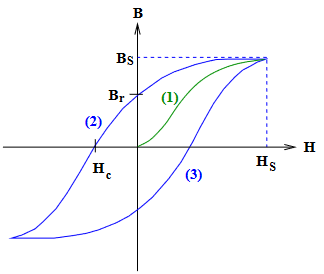
\includegraphics[scale=0.5]{hysterese.png}
    \caption{Schematische Darstellung einer Hystereskurve [1].}
    \label{fig:hysterese}
  \end{figure}
  \FloatBarrier

  Diese Kurve heißt Hystereskurve und ist materialabhängig. Sie stellt den Zusammenhang zwischen magnetischer Feldstärke
  $\vec{H}$ und relativer Permeabilität $\mu_{\symup{r}}$ dar.
  Die Feldstärke $H$ einer Toroidspule lässt sich mittels 
  
  \begin{equation}
    \label{eqn:H}
    H = \frac{nI}{2 \pi r_T}
  \end{equation}
  
  berechnen. $n$ ist die Windungszahl, $r_T$ der Radius der Ringspule und $I$ der angeschlossene Strom.
  
  \subsection{Vorbereitungsaufgabe}
  \subsubsection{Diamagnetismus}
  Diamagnetische Materialien entwickeln in einem externen Magnetfeld ein induziertes Magnetfeld in einer Richtung, die dem 
  äußeren Magnetfeld entgegengesetzt ist. Diamagnetische Materialien haben die Tendenz, aus einem inhomogenen Magnetfeld herauszuwandern.
  Ohne äußeres Magnetfeld haben diamagnetische Materialien kein eigenes Magnetfeld, sie sind nichtmagnetisch.

  \subsubsection{Paramagnetismus}
  Wie der Diamagnetismus beschreibt er das magnetische Verhalten eines Materials, das einem externen Magnetfeld ausgesetzt ist.
  Paramagneten folgen in ihrer Magnetisierung dem äußeren Feld, sodass das Magnetfeld in ihrem Inneren stärker ist als außerhalb.
  Paramagnetische Materialien haben dadurch die Tendenz, in ein Magnetfeld hineingezogen zu werden. Ohne ein äußeres Magnetfeld
  zeigen paramagnetische Materialien keine magnetische Ordnung.

  \subsubsection{Ferromagnetismus}
  Die magnetischen Momente der Atome des Materials neigen dazu, sich parallel auszurichten. Ferromagneten erzeugen entweder selbst
  ein dauerhaftes Magnetfeld oder werden von einem Pol eines äußeren Magnetfelds stark angezogen. Ferromagnetische Materialien sind 
  normalerweise Festkörper.

  \newpage
  \section{Durchführung}
  \label{sec:Durchführung}

  \subsection{Lange Spule und dicke Spule}
  \label{sec:langeSpule}
  Die jeweilige Spule wird an ein Netzgerät angeschlossen. Durch Einstellen des Stroms und der Spannung
  wird ein Magnetfeld erzeugt, das durch eine longitudinale Hallsonde gemessen wird. Dabei werden die Messungen jeweils
  in unterschiedlichen Abständen zum horizontalen Spulenmittelpunkt in der Spule gemessen. Alle Messpunkte liegen jeweils auf
  der Rotationssymetrieachse der Spule.

  \subsection{Helmholtz-Spulenpaar}
  \label{sec:helmholtz}
  Es wird ein Helmholtz-Spulenpaar an ein Netzgerät angeschlossen. Mit Hilfe einer transversalen Hallsonde
  wird die Feldstärke innerhalb und außerhalb der Spule gemessen. Alle Messpunkte liegen wieder auf der Rotationssymetrieachse.
  Zudem wird bei jeder Messreihe der Abstand der Helmholtzspulen verändert.

  \subsection{Ringspule}
  \label{sec:ringspule}
  Es wird eine Toroidspule mit Eisenkern als ferromagnetischer Füllstoff verwendet. Der Strom wird
  auf $10$ Ampere erhöht. Danach wird er wieder auf $0$ Ampere runter gefahren. Die Strom wird umgepolt
  und wieder bis auf $10$ Ampere erhöht. Danach wird der Strom wieder auf $0$ Ampere runter gefahren, umgepolt
  und bis auf $10$ Ampere erhöht. Dies geschieht jeweils in $1$ Ampere-Schritten und währenddessen wird die
  magnetische Feldstärke mit Hilfe einer transversalen Hallsonde gemessen.

  \newpage
  \section{Auswertung}
  \label{sec:Auswertung}
  
  \subsection{Magnetfeld einer kurzen und einer langen Spule}
  \subsubsection{Lange Spule}
  Für eine lange Spule der Länge $l=\SI{0,16}{m}$ mit $n=300$ Windungen, die von einem Strom $I=\SI{1,4}{A}$ durchflossen wird,
  ergeben sich die in (Abbildung 3) dargestellten Messwerte für das Magnetfeld $B$. Die Daten für die Anordnung
  können (Tabelle 1) entnommen werden. Der Theoriewert wurde nach (Gleichung 4) berechnet.
  Der Ursprung der Messung wurde an den linken Rand der jeweiligen Spule gelegt und die Messung wurden von der Mitte der jeweiligen
  Spule ausgehend begonnen.

  \begin{figure}
    \centering
    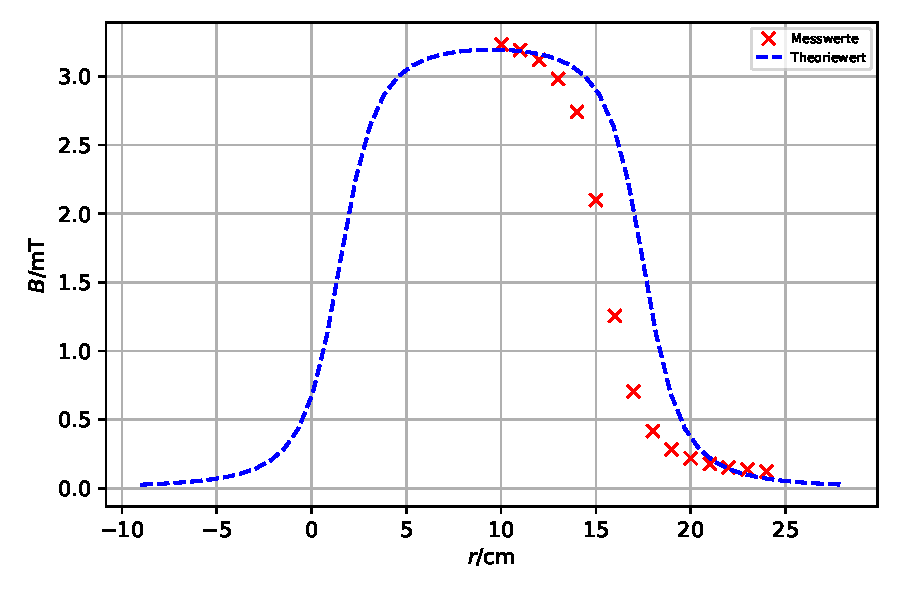
\includegraphics{lange_spule.pdf}
    \caption{Auswertung der Messwerte für die magnetische Feldstärke der langen Spule}
    \label{fig:lange_spule}
  \end{figure}
  \FloatBarrier
  
  Es ist zu erkennen, dass die Messwerte im Grunde dem theoretisch vorher gesagtem Verlauf entsprechen.
  Im Spuleninneren sind sie annähernd konstant und haben nur einen minimalen Unterschied zum Erwartungswert der Theorie.
  Am Rand der Spule ist zudem ein starker Abfall der magnetischen Feldstärke zu beobachten. Für große $r$ nimmt die
  magnetische Feldstärke einen konstanten Wert an, jedoch entspricht dieser nicht dem Wert $B=0$\,mT, 
  der aus der Theorie erwartet wurde.

  \subsubsection{Kurze Spule}
  Für eine kurze Spule der Länge $l=\SI{0.055}{m}$ mit $n=100$ Windungen, die von einem Strom $I=\SI{1,4}{A}$ durchflossen wird,
  ergeben sich die in (Abbildung 4) dargestellt sind. Die Messwerte können (Tabelle 1) entnommen werden.
  Der Theoriewert wurde auch in diesem Fall mit (Gleichung 4) berechnet.

  \begin{figure}
    \centering
    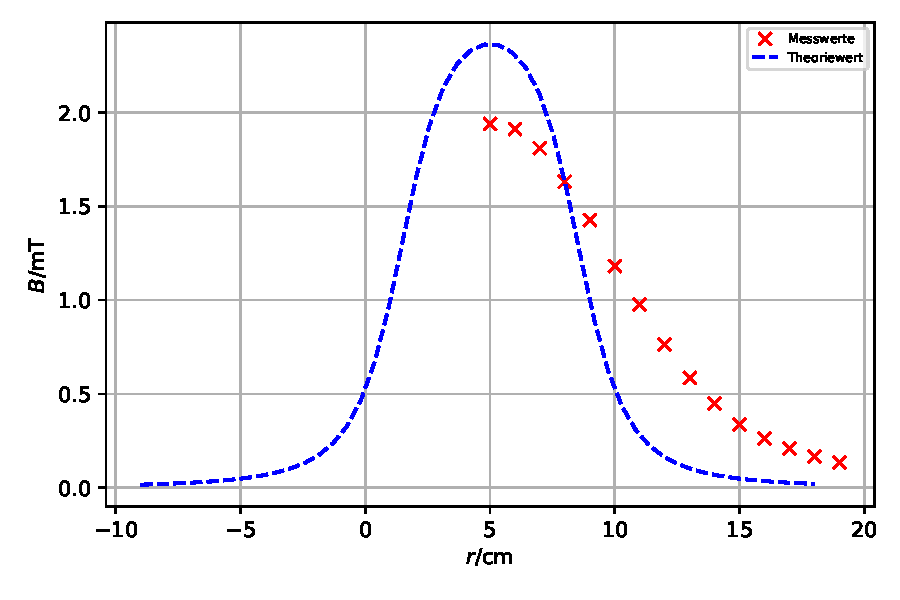
\includegraphics{kurze_spule.pdf}
    \caption{Auswertung der Messwerte für die magnetische 
    Feldstärke der kurzen Spule}
    \label{fig:kurze_spule}
  \end{figure}
  \FloatBarrier

  Der Verlauf der Messwerte für die magnetische Feldstärke zeigt auch hier nahezu, wenn auch leicht abweichend, den
  theoretisch erwarteten Verlauf. Das Feld ist zudem, wie bei einer kurzen Spule auch zu erwarten ist, im Inneren 
  nicht konstant und fällt nach außen hin schnell ab. Zudem lässt sich auch hier, wie schon bei der langen Spule,
  feststellen dass das Feld für große Abstände $r$ nicht gegen Null geht.

  \begin{table}
    \centering
      \caption{Messdaten zur magnetischen Feldstärke einer langen Spule $B_{\symup{l}}$ und einer kurzen Spule $B_{\symup{k}}$}
      \label{tab:einzelne_spulen}
      \begin{tabular}{c c c}
        \toprule
         $r$/cm & $B_{\symup{l}}/$mT & $B_{\symup{k}}/$mT\\
        
        \midrule
        
         5 & - & 1.940\\
         6 & - & 1.911\\
         7 & - & 1.809\\
         8 & - & 1.632\\
         9 & - & 1.426\\
        10 & 3.233 & 1.181\\
        11 & 3.191 & 0.977\\
        12 & 3.121 & 0.764\\
        13 & 2.982 & 0.585\\
        14 & 2.742 & 0.448\\
        15 & 2.098 & 0.335\\
        16 & 1.255 & 0.264\\
        17 & 0.704 & 0.209\\
        18 & 0.416 & 0.166\\
        19 & 0.281 & 0.134\\
        20 & 0.218 & -\\
        21 & 0.177 & -\\
        22 & 0.152 & -\\
        23 & 0.136 & -\\
        24 & 0.123 & -\\
        
        \bottomrule
      \end{tabular}
  \end{table}

  \FloatBarrier

  \newpage
  \subsection{Magnetfeld eines Helmholtzspulenpaares}

  Im folgenden soll die magnetische Feldstärke des Helmholtzspulenpaares in Abhängigkeit
  von der Position auf der Achse, welche durch den Mittelpunkt der beiden Spulen läuft, bestimmt werden.
  Die Spulen besitzen jeweils $n=100$ Windungen und einen Durchmesser von $D=\SI{0,125}{\metre}$, zudem
  werden sie von einem Strom $I=\SI{5}{\ampere}$ durchflossen.
  Daraus ergeben sich die Messwerte (Tabelle 2), (Tabelle 3) und (Tabelle 4).
  In (Abbildung 5), (Abbildung 6) und (Abbildung 7) sind die Messwerte sowie
  die Theoriekurve graphisch dargestellt. Der Ursprung wurde dabei in das Zentrum zwischen den Spulen gelegt.\\\\
  Die Messungen lassen erkennen, dass die gemessenen Werte nur minimal von den Werten der Theorie
  abweichen. Da die Werte insgesamt sehr gut den Verlauf der Kurve der Theorie wiederspiegeln, liegt
  die Annahme nahe, dass die Theorie das reale Feld auch in diesem Bereich sehr gut beschreibt.

  \newpage
  \begin{figure}
    \centering
    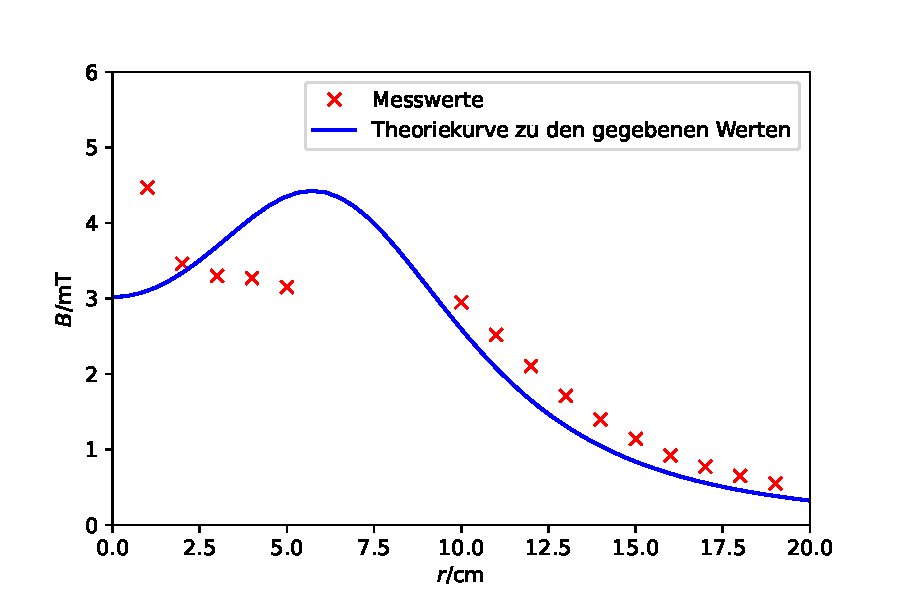
\includegraphics{Helmholtz10.pdf}
    \caption{Messwerte für die magnetische 
              Feldstärke $B$ des Helmholtzspulenpaares
              für den Abstand $r=\SI{0.1}{\metre}$}
    \label{fig:helmholtz1}
  \end{figure}

  \FloatBarrier

  \begin{figure}
    \centering
    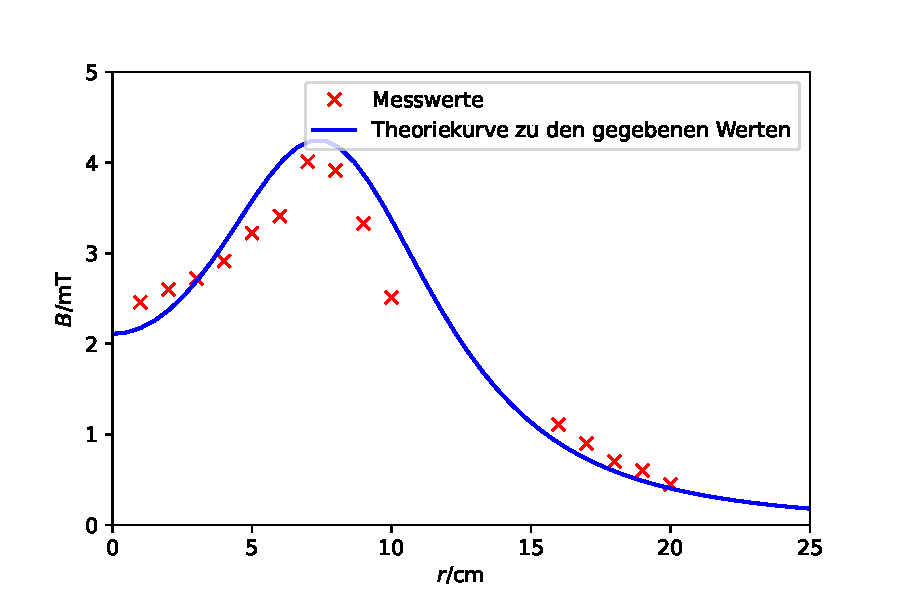
\includegraphics{Helmholtz15.pdf}
    \caption{Messwerte für die magnetische Feldstärke $B$ des Helmholtzspulenpaares
              für den Abstand $r=\SI{0.15}{\metre}$}
    \label{fig:helmholtz2}
  \end{figure}
  
  \FloatBarrier

  \begin{figure}
    \centering
    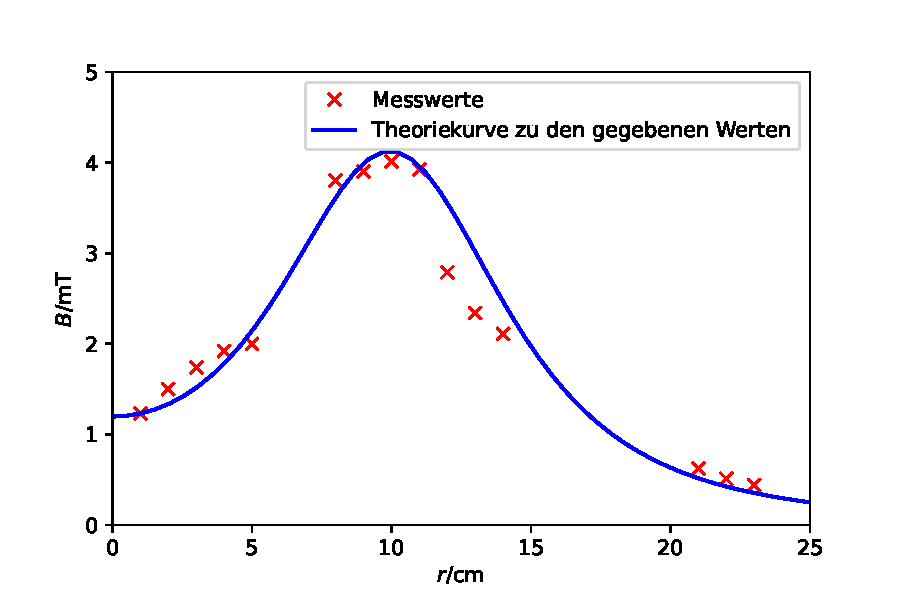
\includegraphics{Helmholtz20.pdf}
    \caption{Messwerte für die magnetische Feldstärke $B$ des 
    Helmholtzspulenpaares für den Abstand $r=\SI{0.2}{\metre}$}
    \label{fig:helmholtz3}
  \end{figure}

  \FloatBarrier

  \newpage
  \begin{table}
    \centering
    \caption{Messdaten zum Magnetfeld des Helmholtzspulenpaar 
      bei einem Abstand von $r=\SI{0.1}{\metre}$}
    \label{tab:helmholtz1}
    \begin{tabular}{c c}
      \toprule
      $B$/mT & $r/$cm\\
      \midrule

      4.47 & 1\\
      3.46 & 2\\
      3.30 & 3\\
      3.27 & 4\\
      3.15 & 5\\
      2.95 & 10\\
      2.52 & 11\\
      2.10 & 12\\
      1.71 & 13\\
      1.40 & 14\\
      1.14 & 15\\
      0.92 & 16\\
      0.77 & 17\\
      0.65 & 18\\
      0.55 & 19\\
      
      \bottomrule
    \end{tabular}
  \end{table}

  \FloatBarrier

  \begin{table}
    \centering
    \caption{Messdaten zum Magnetfeld des Helmholtzspulenpaar 
      bei einem Abstand von $r=\SI{0.15}{\metre}$}
    \label{tab:helmholtz2}
    \begin{tabular}{c c}
      \toprule
      $B$/mT & $r/$cm\\
      \midrule
      2.46 & 1\\
      2.60 & 2\\
      2.72 & 3\\
      2.91 & 4\\
      3.22 & 5\\
      3.41 & 6\\
      4.01 & 7\\
      3.91 & 8\\
      3.33 & 9\\
      2.51 & 10\\
      1.11 & 16\\
      0.90 & 17\\
      0.70 & 18\\
      0.60 & 19\\
      0.45 & 20\\

      \bottomrule
    \end{tabular}
  \end{table}

  \FloatBarrier

  \begin{table}
    \centering
    \caption{Messdaten zum Magnetfeld des Helmholtzspulenpaar 
      bei einem Abstand von $r=\SI{0.20}{\metre}$}
    \label{tab:helmholtz3}
    \begin{tabular}{c c}
      \toprule
      $B$/mT & $r/$cm\\
      \midrule
      1.23 & 1\\
      1.5 & 2\\
      1.74 & 3\\
      1.92 & 4\\
      2.00 & 5\\
      3.8 & 8\\
      3.9 & 9\\
      4.01 & 10\\
      3.92 & 11\\
      2.79 & 12\\
      2.34 & 13\\
      2.11 & 14\\
      0.62 & 21\\
      0.51 & 22\\
      0.44 & 23\\

      \bottomrule
    \end{tabular}
  \end{table}

  \FloatBarrier

  \newpage
  \subsection{Bestimmung des Hysteresekurve einer Toroidspule mit Eisenkern}

  Zur Bestimmung der Hysteriekurve für die Toroidspule mit Eisenkern
  wird die Stromstärke $I$ gegenüber der magnetischen Feldstärke $B$ aufgetragen.
  Daraus folgt der Graph (Abbildung 8). Die gemessenen Daten können 
  der Tabelle (Tabelle 5) entnommen werden.

  \begin{figure}
    \centering
    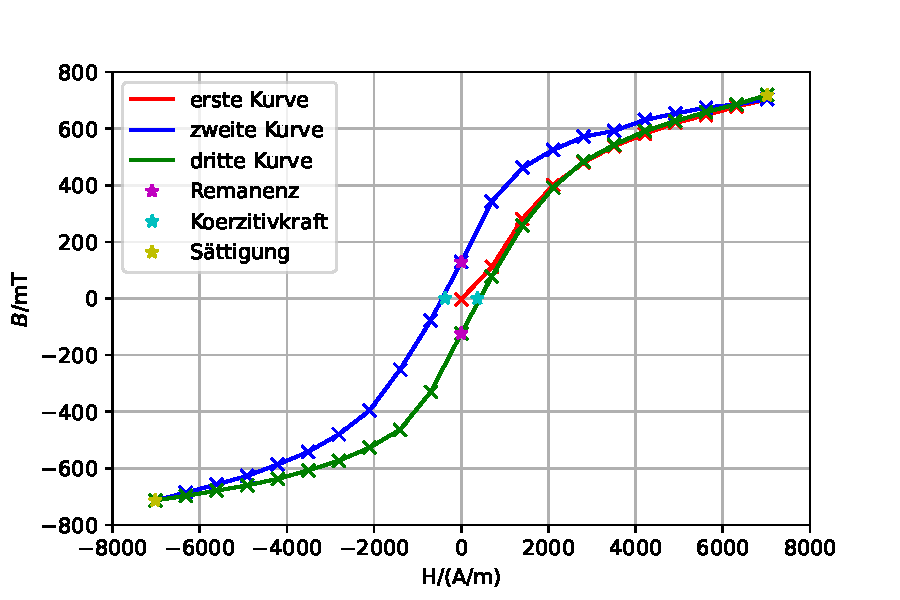
\includegraphics{plot5.pdf}
    \caption{Hysteresekurve der Ringspule}
    \label{fig:hysterese1}
  \end{figure}

  \FloatBarrier

  \begin{figure}
    \centering
    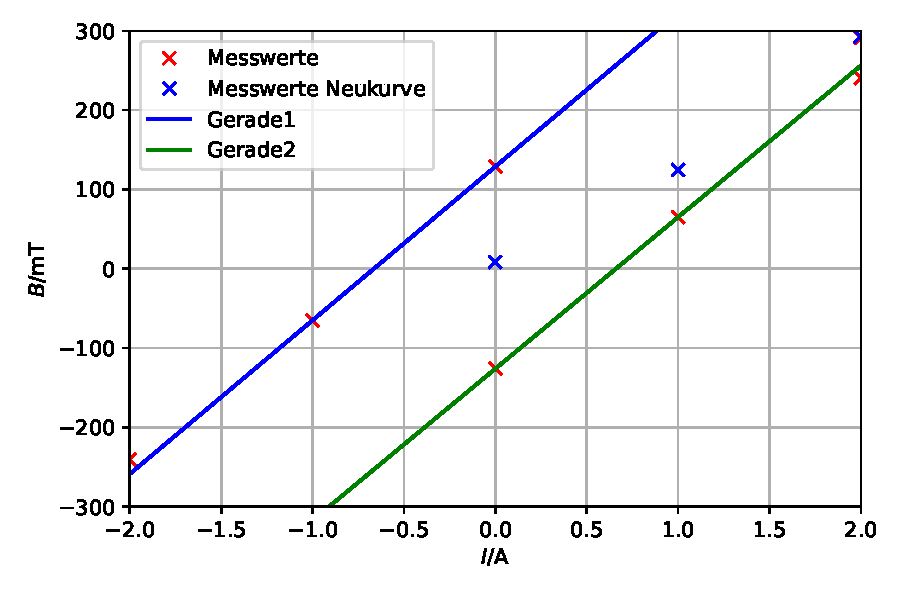
\includegraphics{koerzitiv.pdf}
    \caption{Geraden aus denen die Stromstärke für die Koerzitivfeldstärke bestimmt werden}
    \label{fig:koerzitiv}
  \end{figure}

  \FloatBarrier

  Für die Remanenz sind die Werte $B_{\symup{r}} = \SI{127,5}{\milli\tesla}$ und $B_{\symup{r}}=\SI{-125,2}{\milli\tesla}$
  ablesbar.
  Für den Strom ergibt sich durch berechnung in Python eine Koerzitivfeldstärke von 
  \begin{align}
    H_{\symup{1}}&=-462.3 \text{A/m} & H_{\symup{2}}&=478.4\, \text{A/m}\,.
  \end{align}

  Der Verlauf der Hystereskurve stimmt mit der gegebenen Theoriekurve (Abbildung 8) gut überein,
  jedoch besitzt die gemessene Kurve im Versuch nur eine geringe Sättigung. Insgesamt fällt 
  die Kurve sehr schmall aus im Vergleich zur Theoriekurve.

  \begin{table}
    \centering
    \caption{Messdaten für die magnetische Feldstärke 
            in der Toroidspule in Abhängigkeit der Stromstärke}
    \label{tab:hysterese}
    \begin{tabular}{c c c}
      \toprule
      $I/$A & $B/$mT & $H/\unit{\ampere}/\unit{\m}$\\
      \midrule
      0 & 8.34 & 0\\
      1 & 124.8 & 701.8\\
      2 & 291.0 & 1403.6\\
      3 & 407.8 & 2104.4\\
      4 & 482.9 & 2807.3\\
      5 & 536.7 & 3509.1\\
      6 & 582.6 & 4210.9\\
      7 & 613.8 & 4912.7\\
      8 & 646.8 & 5614.5\\
      9 & 679.9 & 6316.3\\
      10 & 702.1 & 7018.2\\
      9 & 686.5 & 6316.3\\
      8 & 668.3 & 5614.5\\
      7 & 648.6 & 4912.7\\
      6 & 624.3 & 4210.9\\
      5 & 595.3 & 3509.1\\
      4 & 559.7 & 2807.3\\
      3 & 513.5 & 2105.4\\
      2 & 447.2 & 1403.6\\
      1 & 324.5 & 701.8\\
      0 & 134.8 & 0\\
      -1 & -66.96 & -701.8\\
      -2 & -250.4 & -1403.6\\
      -3 & -384.9 & -2105.4\\
      -4 & -472.5 & -2807.3\\
      -5 & -529.3 & -3509.1\\
      -6 & -574.5 & -4210.9\\
      -7 & -619.7 & -4912.7\\
      -8 & -662.2 & -5614.5\\
      -9 & -681.5 & -6316.3\\
      -10 & -702.4 & -7018.2 \\
      -9 & -679.1 & -6316.3\\
      -8 & -661.2 & -5614.5\\
      -7 & -644.8 & -4912.7\\
      -6 & -626.0 & -4210.9\\
      -5 & -590.5 & -3509.1\\
      -4 & -560.0 & -2807.3\\
      -3 & -512.2 & -2105.4\\
      -2 & -443.6 & -1403.6\\
      -1 & -321.4 & -701.8\\
      0 & -122.3 & 0\\
      1 & 65.0 & 701.8\\
      2 & 240.0 & 1403.6\\
      3 & 374.0 & 2105.4\\
      4 & 467.8 & 2807.3\\
      5 & 534.5 & 3509.1\\
      6 & 575.1 & 4210.9\\
      7 & 611.1 & 4912.7\\
      8 & 648.2 & 5614.5\\
      9 & 676.2 & 6316.3\\
      10 & 710.4 & 7018.2\\
      
      \bottomrule
    \end{tabular}
  \end{table}

  
  \newpage
  \section{Diskussion}

  \subsection{Lange und kurze Spule}

  Die Messwerte weisen leichte Abweichungen von der Theoriekurve auf. Dies kann daran liegen, dass
  das Stativ, an dem die Hallsonde befestigt wurde, sehr wackelig war und dadurch beim Verschieben die Sonde sich bewegt haben
  und nicht mehr horizontal zur Spule ausgerichtet war. Im Grunde sind die Werte aber trotzdem gut und stimmen zum großen 
  Teil mit der Theorie überein.\\
  Die kurze Spule weist in der Theorie, im Vergleich zu der langen Spule, keine Homogenität in ihrer Mitte auf. Aus Abbildung 4
  ist deutlich zu sehen, dass es nur einen Punkt gibt, an dem das magnetische Feld am stärksten ist, im Gegensatz zu einer langen
  Spule, bei der es ein längerer Abschnitt wäre. Die Homogenität im inneren einer Spule ist nur bei ausreichender Länge annähernd
  nachweisbar, sodass in diesem Fall die Randeffekte überwiegen.

  \subsection{Helmholtzspulenpaar}

  Die Messwerte weisen auch hierbei nur sehr kleine Abweichungen von der Theorie auf. Dies kann dadurch begründet werden,
  dass die Helmholtzspulen während des Betriebs heiß werden und dadurch der Widerstand erhöht wird. Zudem ist auch bei diesem
  Versuchsteil der Aufbau sehr wackelig war, was natürlich auch wieder dazu geführt haben könnte, dass die Messwerte leicht
  abweichen.\\
  Die Besonderheit des Helmholtzspulenpaares ist die näherungsweise Homogenität zwischen den beiden Spulen, wenn der Abstand
  dem Radius entspricht. Außerhalb des Spulenpaares treten wieder Randeffekte auf, sodass das Feld wie auch bei den anderen 
  Spulen schnell stark abfällt. Bei den anderen Abständen der beiden Spulen ist das magnetische Feld immer noch näherungsweise
  homogen, nun aber in der Mitte ein wenig schwächer.

  \subsection{Hysteresekurve}

  Die Hysteresekurve, die durch die Messwerte graphisch dargestellt wurde, stimmt sehr gut mit der Theoriekurve überein.
  Leider gibt es für die Kurve keine Theoriewerte, die zum Vergleich herangezogen werden könnten.

  \newpage
  \section{Literaturverzeichnis}
    [1] TU Dortmund. V308: Spulen und Magnetfelder. 2022.
\end{document}
